\section{Pengenalan Android Dan Android Studio}
\subsection{Android}
 \begin{figure}[H]
    \centering
    
\includegraphics[width=0.9\textwidth]{figures/android.png}
    \caption{Logo Android}
    \label{print}
    \end{figure}
    
    \par Android adalah sistem operasi yang dirancang oleh Google dengan basis kernel Linux untuk mendukung kinerja perangkat elektronik layar sentuh, seperti tablet atau smartphone. Jadi, android digunakan dengan sentuhan, gesekan ataupun ketukan pada layar gadget anda.\\
    \par Android  salah satu sistem operasi atau \textit{operating system} berbasis \textit{mobile} yang sangat banyak di gunakan sekarang ini. Utamanya pada telepon pintar \textit{(smartphone)} ataupun tablet.\\
    \par Android bersifat \textit{open source} atau bebas digunakan, dimodifikasi, diperbaiki dan didistribusikan oleh para pembuat ataupun pengembang perangkat lunak. Dengan sifat \textit{open source} perusahaan teknologi bebas menggunakan OS ini diperangkatnya tanpa lisensi alias gratis.
    \par Kelebihan Android yaitu sebagai berikut :
    \begin{enumerate}
        \item Merupakan Sistem Operasi Open Source
\par Siapa saja bisa menggunakannya secara gratis. Para \textit{developer} atau pengembang dimudahkan untuk mengoptimalkan dan mengembangkan OS ini untuk \textit{smartphone} yang dibuatnya.

\item Memiliki Banyak Dukungan Aplikasi
\par Hal ini juga tidak lepas dari sifat Android yang merupakan sistem operasi \textit{Open Source}. Pengembang pun diizinkan untuk mengembangkan aplikasi berbasis source code dari Android.

\par Oleh karena itu, jika Anda masuk ke \textit{Play Store}, akan ditemukan banyak sekali ribuan aplikasi yang sesuai dengan kebutuhan pengguna.

\item Mudah dimodifikasi
\par Banyak komponen yang bisa Anda atur ulang atau dimodifikasi, mulai dari ROM  hinga custom \textit{overclock} pada sistem operasi. Hal ini bisa berpengaruh terhadap performa ponsel pintar berbasis Android agar bisa bekerja lebih cepat dan sesuai dengan keinginan.
\end{enumerate}
\par Kekurangan Android yaitu sebagai berikut :
\begin{enumerate}
    \item  Kerja sistemnya cukup berat
    \par Hal ini menyebabkan banyak memori yang dibutuhkan, baik RAM maupun ROM. Bagi \textit{smartphone} yang memiliki RAM dan ROM berkapasitas kecil, tentunya akan menghambat performanya.
    \item Hasil modifikasi sering menyebabkan sistem bekerja tidak stabil dan kurang optimal
    \par Adakalanya hasil modifikasi mengakibatkan OS menjadi sedikit lelet dan kurang responsif. Nantinya, bisa berpengaruh pada hardware sehingga menjadi cepat panas dan kapasitas memori lebih mudah bocor.
    \item Kurang responsif jika disandingkan dengan spesifikasi hardware yang tidak baik
    \par Hal tersebut berkaitan dengan kapasitas RAM, ROM, dan kecepatan prosesor yang digunakan pada \textit{smartphone.}
\end{enumerate}
\subsection{Perkembangan Android}
    \begin{figure}[H]
    \centering
    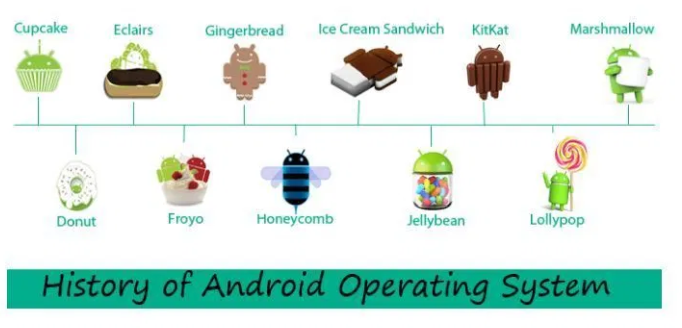
\includegraphics[width=0.9\textwidth]{figures/android2.png}
    \caption{Perkembangan Android}
    \label{print}
    \end{figure}

\par Sejak tahun 2009, Android mulai dikembangakn dengan kode yang dinamai berdasarkan makanan pencuci mulut. Tiap versi dirilis sesuai dengan urutan abjad.
\begin{enumerate}
    \item Astro 1.0
    \par Versi ini pertama kali dirilis pada 23 September 2008 yang awalnya akan dinamai dengan nama “Astro” saja. Namun karena alasan hak cipta dan trademark, nama ini tidak jadi disematkan pada versi pertama ini. Versi Astro 1.0 pertama kali digunakan oleh smartphone HTC Dream.
    \item Bender 1.1
    \par Bender 1.1 dirilis pada 9 Februari 2009. Lagi-lagi, versi dari OS ini mengalami masalah penamaan yang serupa dengan versi sebelumnya. Awalnya, versi ini diberi nama Bender dan dirilis untuk perangkat T-Mobile G1 saja.
    \item Cupcake 1.5
    \par Cupcake 1.5 dirilis pada 30 April 2009. Dimulai dari versi ini, penamaan menggunakan nama makanan pencuci mulut. Karena merupakan versi ketiga, makan penamaannya dimulai dengan huruf “C” dan “Cupcake” menjadi nama resminya.
    \item Donut 1.6
    \par Versi yang dirilis pada 15 September 2009 ini memiliki peningkatan pada fitur pencarian dan UI yang lebih user friendly. Donut 1.6 sudah mendukung teknologi CDMA/EVDO, 802.1 x, VPNs.
    \item Eclair 2.0 – 2.1
    \par Eclair 2.0 – 2.1 dirilis pada 3 Desember 2009 dan untuk pertama kalinya membawa fitur baru, yaitu Google Maps yang dapat membantu pengguna dalam bepergian.
    \item Froyo 2.2
    \par Froyo atau disingkat dari frozen yoghurt merupakan versi Android yang rilis pada 20 Mei 2010.

\par Perubahan umumnya antara lain adalah adanya dukungan Adobe Flash 10.1, kecepatan kinerja, intergrasi V8 JavaScript engine, pemasangan aplikasi dalam SD Card, kemampuan Wi-Fi Hotspot portable, dan kemampuan auto update dalam aplikasi Android Market.

\item Gingerbread 2.3
\par Versi ini dirilis pada 6 Desember 2010 dan terdapat perubahan dalam peningkatan kemampuan gaming, peningkatan fungsi copy paste, User Interface, dukungan format video VP8 dan WebM, hingga dukungan jumlah kamera lebih dari satu.\\
\\
\\
\item Honeycomb 3.0/3.1
\par Versi yang diluncurkan pada 22 Februari 2011 ini merupakan OS yang didesain khusus untuk pengoptimalan penggunaan pada tablet PC. Versi Honeycomb ini juga mendukung multi prosesor dan akselerasi hardware untuk grafis.

\item Ice Cream Sandwich 4.0
\par Ice Cream Sandwich 4.0 diluncurkan tanggal 19 Oktober 2011 dan membawa fitur Honeycomb untuk smartphone dengan membawa fitur brau, seperti membuka kunci dengan pengenala wajah, perangkat tambahan fotografi, hingga berbagi informasi menggunakan NFC.
\item Jelly Bean 4,1/4.2/4.3
\par Di tahun 2012, android mengeluarkan versi Jelly Bean. Lewat versi Jelly Bean (4.1) Google mulai menerapkan teknologi asisten digital Google Now yang bisa diakses langsung dari homescreen.

\par Pada versi 4.2 terdapat fitur photo sphere untuk panorama, daydream sebagai screensaver, power control, dsb. Sedangkan versi 4.3 merupakan pembaharuan dari versi sebelumnya.
\item KitKat 4.4
\par KitKat 4.4 diluncurkan pada 3 September 2013. Versi yang sebelumnya bernama Key Lime Pie ini membawa peningkatan yang cukup signifikan karena Google lebih fokus meningkatkan user experience.

\par Versi ini dioptimalkan untuk berjalan pada rentang yang lebih besar dari versi Android sebelumnya. Disarankan perangkat harus memiliki minimal RAM 512 MB.

\item Lollipop 5.0
\par Versi yang diluncurkan pada 12 November 2014 ini tersedia secara resmi melalui over the air (OTA). Perubahan yang paling menonjol dalam versi ini adalah User Interface yang didesain ulang dan dibangun dengan “material design”.
\item Marshmallow 6.0
\par Sistem operasi ini membawa banyak fitur canggih, mulai dari Doze untuk menghemat baterai, dukungan USB tipe C, percobaan multi window, sensor sidik jari untuk buka kunci layar, hingga pengguna bisa memakai dua aplikasi berbeda dalam satu layar.
\item Nougat 7.0
\par Versi ini merupakan salah satu upgrade terbesar dalam sistem operasi Android. Nougat 7.0 merupakan pengembangan dari Marshmallow yang meningkatkan performa dan interface yang lebih intuitif.\\
\\
\item Oreo 8.0
\par Orea 8.0 dirilis pada 2017 dengan menambah lebih banyak fitur multi tasking dan perombakan bagian notifikasi. Pengguna bisa mengatur mana saja notifikasi yang ingin ditampilkan.

\par Tampilan UI-nya juga lebih rapi dan segar, serta difokuskan untuk memudahkan pengguna mengakses aplikasi dan mencari informasi.
\item Pie 9.0
\par Versi yang diluncurkan pada Agustus 2018 ini mengganti tiga tombol navigasi dengan tombol tunggal berbentuk elips. Android Pie disokong dengan kemampuan kecerdasan buatan (AI) yang menjadikannya bisa mempelajari pola penggunaan secara otomatis.
\end{enumerate}
\subsection{Android Studio}
\begin{figure}[H]
    \centering
    
\includegraphics[width=0.9\textwidth]{figures/android3.jpeg}
    \caption{Logo Android Studio}
    \label{print}
    \end{figure}
\par Android Studio adalah Lingkungan Pengembangan Terpadu (\textit{Integrated Development Environment}/IDE) resmi untuk pengembangan aplikasi Android, yang didasarkan pada IntelliJ IDEA. Selain sebagai editor kode dan fitur developer IntelliJ yang andal, Android Studio menawarkan banyak fitur yang meningkatkan produktivitas Anda dalam membuat aplikasi Android, seperti:
\begin{enumerate}
    \item Sistem build berbasis Gradle yang fleksibel
    \item Emulator yang cepat dan kaya fitur
    \item Lingkungan terpadu tempat Anda bisa mengembangkan aplikasi untuk semua perangkat Android.
    \item Terapkan Perubahan untuk melakukan push pada perubahan kode dan resource ke aplikasi yang sedang berjalan tanpa memulai ulang aplikasi.
    \item Template kode dan integrasi GitHub untuk membantu Anda membuat fitur aplikasi umum dan mengimpor kode sampel.
    \item Framework dan fitur pengujian yang lengkap.
    \item Fitur lint untuk merekam performa, kegunaan, kompatibilitas versi, dan masalah lainnya.
    \item Dukungan C++ dan NDK.
    \item Dukungan bawaan untuk Google Cloud Platform, yang memudahkan integrasi Google Cloud Messaging dan App Engine.
\end{enumerate}

\subsection{Struktur \textit{Project}}
\par Setiap \textit{project} di Android Studio berisi satu atau beberapa modul dengan file kode sumber dan \textit{file resource}. Jenis modul meliputi:
\begin{enumerate}
    \item Modul aplikasi Android.
    \item Modul library.
    \item Modul Google App Engine.
\end{enumerate}
\begin{figure}[H]
    \centering
    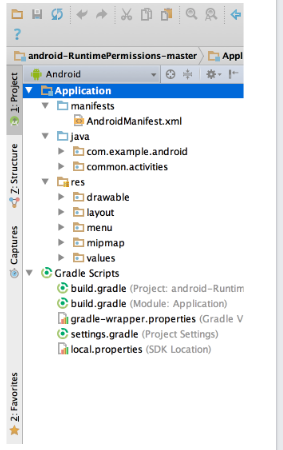
\includegraphics[width=0.5\textwidth]{figures/android4.png}
    \caption{ File project Dalam Tampilan Android}
    \label{print}
    \end{figure}
\par Secara \textit{default}, Android Studio menampilkan \textit{file project} Anda dalam tampilan \textit{project} Android, seperti yang ditunjukkan pada gambar. Tampilan ini disusun menurut modul untuk memberikan akses cepat ke file sumber utama \textit{project}.
\par Semua\textit{ file build } terlihat di tingkat teratas di bagian\textit{ Gradle Script} dan setiap modul aplikasi berisi folder berikut:
\begin{enumerate}
    \item manifes: Berisi file AndroidManifest.xml.
    \item java: Berisi file kode sumber Java, termasuk kode pengujian JUnit.
    \item res: Berisi semua resource non-kode, seperti tata letak XML, string UI, dan gambar bitmap.
    \end{enumerate}
    
\par Struktur \textit{project} Android pada disk berbeda dengan representasi tersatukan ini. Untuk melihat struktur \textit{file project} sebenarnya, pilih \textit{Project} dari menu d\textit{rop-down Project}.

\par Menyesuaikan tampilan\textit{ file project} untuk berfokus pada aspek spesifik dari pengembangan aplikasi. Misalnya, memilih tampilan \textit{Problems} pada \textit{project} akan menampilkan link ke \textit{file} sumber yang berisi \textit{error coding} dan sintaks yang dikenali, seperti tag penutup elemen XML yang tidak ada dalam file tata letak.
\begin{figure}[H]
    \centering
    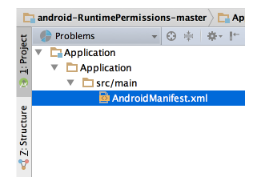
\includegraphics[width=0.9\textwidth]{figures/android5.png}
    \caption{ File Project Dalam Tampilan Problems}
    \label{print}
    \end{figure}
\subsection{Antarmuka Pengguna}
\par endela utama Android Studio terdiri dari beberapa area logis yang diidentifikasi dalam gambar berikut :
\begin{figure}[H]
    \centering
    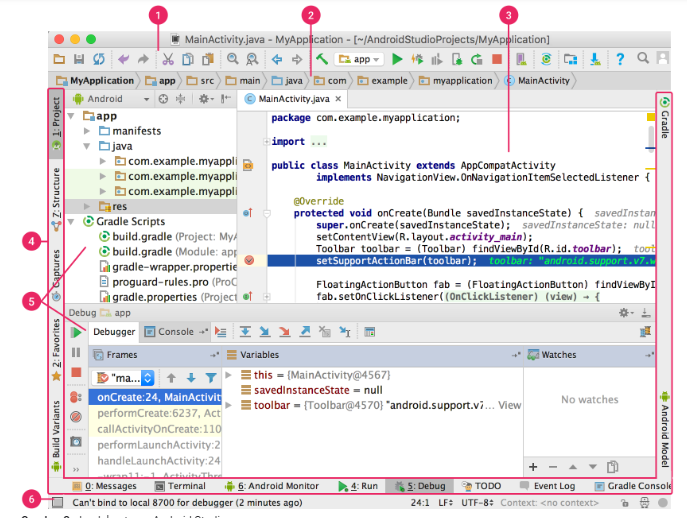
\includegraphics[width=0.9\textwidth]{figures/android6.png}
    \caption{ Jendela utama Android Studio}
    \label{print}
    \end{figure}

\begin{enumerate}
    \item Toolbar memungkinkan  melakukan berbagai tindakan, termasuk menjalankan aplikasi dan meluncurkan fitur Android.
    \item Menu navigasi membantu menjelajah project dan membuka file untuk diedit. Menu ini memberikan tampilan struktur yang lebih ringkas yang terlihat di jendela Project.
    \item Jendela editor adalah tempat membuat dan memodifikasi kode. Tergantung jenis file yang ada, editor ini dapat berubah. Misalnya, saat menampilkan file tata letak, editor akan menampilkan Layout Editor.
    \item Panel jendela fitur berada di sisi luar jendela IDE dan berisi tombol-tombol yang memungkinkan Anda memperluas atau menciutkan setiap jendela fitur.
    \item Jendela fitur memberi akses ke tugas tertentu seperti pengelolaan project, penelusuran, kontrol versi, dan banyak lagi.Dapat memperluas dan menciutkan jendela ini.
    \item Status bar menampilkan status \textit{project} dan IDE itu sendiri, serta semua peringatan atau pesan.
\end{enumerate}
\par Kita dapat mengatur jendela utama untuk memperluas ruang layar dengan menyembunyikan atau memindahkan toolbar dan jendela fitur. Kita juga dapat menggunakan pintasan keyboard untuk mengakses sebagian besar fitur IDE.

\par Selain itu kita dapat menelusuri kode sumber, database, tindakan, elemen antarmuka pengguna, dan sebagainya kapan saja, dengan menekan tombol Shift dua kali, atau mengklik kaca pembesar di sudut kanan atas jendela Android Studio. Tips ini sangat berguna jika, misalnya, mencoba menemukan tindakan IDE tertentu yang lupa cara memicunya.
\subsection{Jendela Fitur}
\par Sebagai ganti menggunakan perspektif preset, Android Studio mengikuti konteks dan otomatis menampilkan jendela fitur yang relevan saat bekerja. Secara default, jendela fitur yang paling umum digunakan disematkan ke panel jendela fitur di tepi jendela aplikasi.
\begin{enumerate}
    \item Untuk memperluas atau menciutkan jendela fitur, klik nama fitur di panel jendela fitur. Dapat menarik, menyematkan, melepaskan sematan, memasang, dan melepas jendela fitur.
    \item Untuk kembali ke tata letak jendela \textit{fitur default} saat ini, klik Window kemudian\textit{ Restore Default Layout} atau sesuaikan tata letak default dengan mengklik Window kemudian \textit{Store Current Layout as Default.}
    \item Untuk menampilkan atau menyembunyikan seluruh panel jendela alat, klik ikon jendela  di pojok kiri bawah jendela Android Studio.
    \item Untuk menemukan jendela alat tertentu, arahkan kursor ke atas ikon jendela dan pilih jendela alat tersebut dari menu.Kita juga bisa menggunakan pintasan keyboard untuk membuka jendela alat dengan mencantumkan pintasan jendela paling umum.
    \begin{figure}[H]
    \centering
    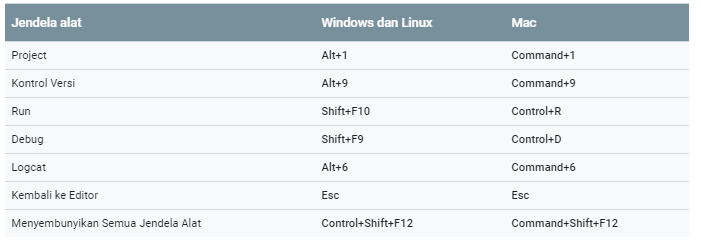
\includegraphics[width=1\textwidth]{figures/android7.png}
    \caption{ Pintasan keyboard Ke Beberapa Jendela Alat yang Berguna.}
    \label{print}
    \end{figure}
\end{enumerate}

\par Jika ingin menyembunyikan semua toolbar, jendela alat, dan tab editor, klik\textit{ View }lalu Enter \textit{Distraction Free Mode.} Langkah ini akan mengaktifkan \textit{Distraction Free Mode}. Untuk keluar dari \textit{Distraction Free Mode}, klik View kemudian  Exit \textit{Distraction Free Mode}.\\
\par Kita dapat menggunakan Speed Search untuk menelusuri dan memfilter di dalam sebagian besar jendela fitur pada Android Studio. Untuk menggunakan \textit{Speed Search}, pilih jendela alat, lalu ketik kueri penelusuran Anda.

\subsection{Pelengkapan kode}
\par Android Studio memiliki tiga jenis pelengkapan kode, yang dapat diakses menggunakan pintasan keyboard.
 \begin{figure}[H]
    \centering
    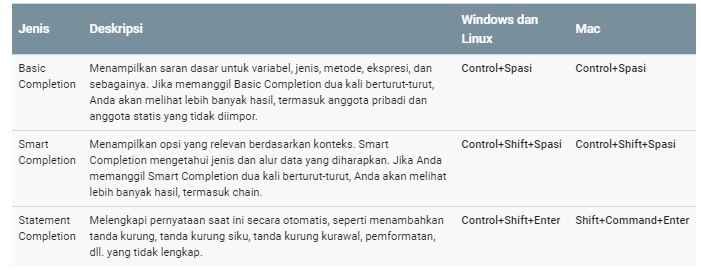
\includegraphics[width=1\textwidth]{figures/android8.png}
    \caption{ Pintasan keyboard untuk Pelengkapan Kode.}
    \label{print}
    \end{figure}
    
\subsection{Navigasi}
\par Berikut ini beberapa tips untuk membantu menjelajah di dalam Android Studio.
\begin{enumerate}
    \item Beralih antar \textit{file} yang baru saja diakses menggunakan tindakan \textit{Recent Files.} Tekan Control+E (Command+E) untuk memunculkan tindakan \textit{Recent Files}. Secara default, file yang terakhir diakses akan dipilih. Anda juga dapat mengakses jendela fitur mana saja melalui kolom kiri dalam tindakan ini.
    \item Lihat struktur file saat ini menggunakan tindakan File \textit{Structure}. Munculkan tindakan\textit{ File Structure }dengan menekan Control+F12 (Command+F12). Dengan tindakan ini,dapat membuka bagian mana pun dari file saat ini dengan cepat.
    \item Telusuri dan buka\textit{ class }tertentu dalam \textit{project} menggunakan tindakan N\textit{avigate to Class}. Munculkan tindakan ini dengan menekan Control+N (Command+O). \textit{Navigate to Class } mendukung ekspresi canggih, termasuk camel humps, jalur, baris navigasi ke, pencocokan nama tengah, dan banyak lagi. Jika Anda memanggilnya dua kali berturut-turut, hasil dari \textit{class project} akan ditampilkan.
    \item Buka file atau folder menggunakan tindakan \textit{Navigate to File.} Munculkan tindakan\textit{ Navigate to File} dengan menekan Control+Shift+N (Command+Shift+O). Untuk menelusuri folder dan bukan file, tambahkan / (garis miring) di akhir ekspresi Anda.
    \item Buka metode atau kolom menurut nama menggunakan tindakan \textit{Navigate to Symbol.} Munculkan tindakan \textit{Navigate to Symbol} dengan menekan Control+Shi\\ft+Alt+N (Command+Option+O).
    \item Temukan semua bagian kode yang merujuk ke\textit{ class}, metode, kolom, parameter, atau pernyataan di posisi kursor saat ini dengan menekan Alt+F7 (Option+F7).
\end{enumerate}
\subsection{Gaya dan Pemformatan}
\par Saat Anda mengedit, Android Studio otomatis menerapkan pemformatan dan gaya seperti yang ditentukan dalam setelan gaya kode Anda. Anda dapat menyesuaikan setelan gaya kode menurut bahasa pemrograman, termasuk menentukan konvensi untuk tab dan indentasi, spasi, penggabungan, tanda kurung kurawal, dan baris kosong. Untuk menyesuaikan setelan gaya kode Anda, klik File > Settings > Editor > Code Style (Preferences > Editor > Code Style).
\par Meskipun IDE otomatis menerapkan pemformatan selagi bekerja, bisa memanggil tindakan Reformat \textit{Code} secara eksplisit dengan menekan Control+Alt+L (Opt+C\\ommand+L), atau otomatis mengindentasi semua baris dengan menekan Control+Alt\\+I (Control+O\\ption+I).
    \begin{figure}[H]
    \centering
    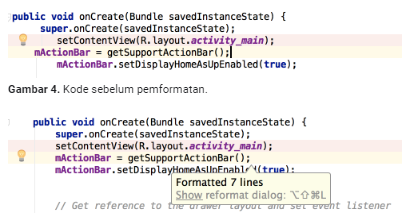
\includegraphics[width=1\textwidth]{figures/android9.png}
    \caption{  Kode Setelah Pemformatan}
    \label{print}
    \end{figure}
\subsection{\textit{Sistem build Gradle}}
\par Android Studio menggunakan Gradle sebagai dasar dari sistem build, dengan lebih banyak kemampuan khusus Android yang disediakan oleh plugin Android untuk Gradle. Sistem\textit{ build }ini berjalan sebagai fitur terintegrasi dari menu Android Studio, dan terpisah dari\textit{ command line} dapat menggunakan fitur-fitur sistem \textit{build} untuk:
\begin{enumerate}
    \item Menyesuaikan, mengonfigurasi, dan memperluas proses pembuatan \textit{build.}
    \item Membuat banyak APK untuk aplikasi, dengan berbagai fitur yang menggunakan \textit{project }dan modul yang sama.
    \item Menggunakan kembali kode dan \textit{resource} di seluruh set sumber.
\end{enumerate}
\par Berkat fleksibilitas Gradle, dapat mencapai semua ini tanpa mengubah file sumber inti aplikasi. File \textit{build} Android Studio diberi nama \textit{build.gradle.} File tersebut adalah file teks biasa yang menggunakan sintaks Groovy untuk mengonfigurasi\textit{ build }dengan elemen yang disediakan oleh plugin Android untuk Gradle. Setiap \textit{project} memiliki satu file build tingkat atas untuk seluruh \textit{project }dan file \textit{build }tingkat modul terpisah untuk setiap modul. Saat Anda mengimpor\textit{ project }yang ada, Android Studio akan otomatis menghasilkan file\textit{ build }yang diperlukan.
\subsection{Fitur Profil dan Debug}
Android Studio membantu menjalankan proses debug dan meningkatkan performa kode, termasuk proses debug inline dan fitur analisis performa.
\begin{enumerate}
    \item Proses debug inline
    \par Gunakan proses debug inline untuk menyempurnakan panduan kode  dalam tampilan debugger dengan verifikasi inline untuk referensi, ekspresi, dan nilai variabel. Informasi debug inline meliputi:
    \begin{enumerate}
        \item Nilai variabel inline
        \item Objek perujuk yang merujuk ke objek terpilih
        \item Nilai yang dihasilkan metode
        \item Ekspresi operator dan lambda
        \item Nilai tooltip
    \begin{figure}[H]
    \centering
    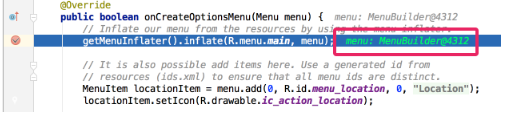
\includegraphics[width=1\textwidth]{figures/android10.png}
    \caption{Nilai Variabel Inline}
    \label{print}
    \end{figure}
    \end{enumerate}
    \par Untuk mengaktifkan proses debug inline, di jendela Debug, klik Settings dan centang kotak \textit{Show Values Inline.}\\
    \\
    \item Akses file data
    \par Android SDK Tools, seperti\textit{ Systrace} dan \textit{logcat,} menghasilkan data performa dan proses debug untuk analisis aplikasi secara mendetail.

    \par Untuk menampilkan file data yang dihasilkan, buka jendela alat Captures. Pada daftar file yang dihasilkan, klik dua kali file untuk melihat data. Klik kanan sembarang file .hprof untuk mengonversinya ke dalam format file standar Menyelidiki penggunaan RAM.
    \item Pemeriksaan kode
    \par Setiap kali  mengompilasi program, Android Studio akan otomatis menjalankan Lint yang telah dikonfigurasi dan pemeriksaan IDE lainnya untuk memudahkan mengidentifikasi serta memperbaiki masalah kualitas struktur kode.

    \par Fitur Lint memeriksa file sumber \textit{project} Android  untuk menemukan potensi bug dan peluang pengoptimalan guna mencapai ketepatan, keamanan, performa, kegunaan, aksesibilitas, serta internasionalisasi.
     \begin{figure}[H]
    \centering
    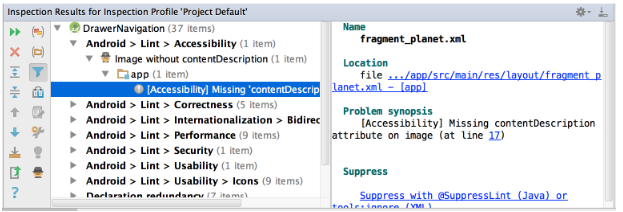
\includegraphics[width=1\textwidth]{figures/android11.png}
    \caption{Hasil pemeriksaan Lint di Android Studio}
    \label{print}
    \end{figure}
    \par Selain pemeriksaan Lint, Android Studio juga menjalankan pemeriksaan kode IntelliJ dan memvalidasi anotasi untuk menyederhanakan alur kerja coding.
\end{enumerate}
\subsection{Anotasi di Android Studio}
\par Android Studio mendukung anotasi variabel, parameter, dan nilai kembalian untuk membantu merekam bug, seperti pengecualian \textit{pointer null} dan konflik jenis \textit{resource}. Android SDK Manager mengemas library Support-Annotations di Android Support Repository untuk digunakan dengan Android Studio. Android Studio memvalidasi anotasi yang sudah dikonfigurasi selama pemeriksaan kode.
\subsection{Pesan Log}
\par Saat membuat dan menjalankan aplikasi dengan Android Studio, dapat melihat output adb dan pesan log perangkat di jendela Logcat.
\subsection{\textit{Interfaces} dan Struktur \textit{Project} Android Studio}
\par \textit{Interfaces} dan struktur \textit{project} android studio ini sangat penting perlu diketahui. Mengapa? Karena agar pada saat memprogram kita tidak bingung dari berbagai \textit{interfaces} dan struktur \textit{project} yang sedia. Beriku penjelesannya:
\begin{enumerate}
    \item Antar Muka \textit{(Interface )} Android Studio
     \begin{figure}[H]
    \centering
    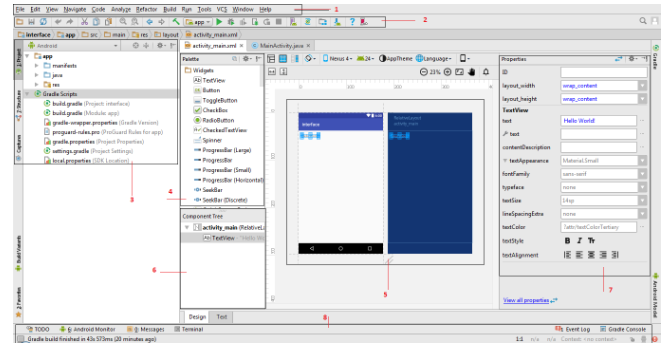
\includegraphics[width=1\textwidth]{figures/android13.png}
    \caption{\textit{Interfaces} Android Studio}
    \label{print}
    \end{figure}
    
    \item  Menu Bar 
    \par Seperti pada aplikasi lain Menu bar merupakan bagian antar muka \textit{(interface)} pengguna yang berisi perintah dan opsi yang dapat dipilih untuk mengeksekusi suatu perintah.
     \begin{figure}[H]
    \centering
    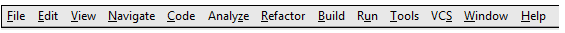
\includegraphics[width=1\textwidth]{figures/android14.png}
    \caption{Menu Bar Android Studio}
    \label{print}
    \end{figure}
    
    \item  Tool Bar
    \par Dengan tool bar kita bisa mempercepat perintah pada sebuah aplikasi.
    \begin{figure}[H]
    \centering
    
\includegraphics[width=1\textwidth]{figures/android15.png}
    \caption{Tool Bar Android Studio}
    \label{print}
    \end{figure}
    
    \\
    \\
    \\
    \\
    \item Struktur\textit{ Project}
    \par Pada bagian ini akan ditampilkan folder-folder dari sebuah \textit{project} aplikasi android yang dibuat menggunakan android studio.
    \begin{figure}[H]
    \centering
    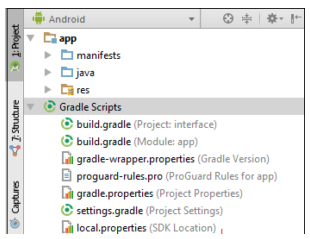
\includegraphics[width=0.5\textwidth]{figures/android16.png}
    \caption{Struktur \textit{Project} Android Studio}
    \label{print}
    \end{figure}
    
    \item \textit{Pallete}
    \par Di\textit{ pallete} tersedia semua\textit{ tools} untuk membuat aplikasi android dan enaknya lagi untuk menggunakannya cukup dengan mendrag and drop ke design android.
    \begin{figure}[H]
    \centering
    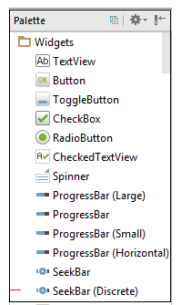
\includegraphics[width=0.4\textwidth]{figures/android17.png}
    \caption{Pallet Android Studio}
    \label{print}
    \end{figure}
    
    \item\textit{ Design} Android
    \par Tempat ini digunakan untuk mendesign layout aplikasi dengan cara drag and drop (tidak mengetikan script xml).
    \begin{figure}[H]
    \centering
    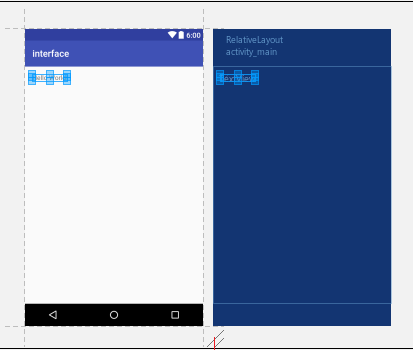
\includegraphics[width=0.7\textwidth]{figures/android18.png}
    \caption{Design Android Studio}
    \label{print}
    \end{figure}
    
    \item \textit{Tree}
    \par Setelah kita menggunakan \textit{tools} yang ada di pallete maka akan ditampilkan pada component tree misal kita mendrag TextView (widget untuk membuat teks) ke design android. Maka nanti ditampilkan di component tree TextView. 
    \begin{figure}[H]
    \centering
    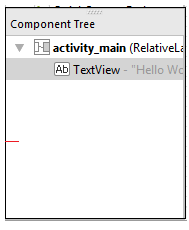
\includegraphics[width=0.4\textwidth]{figures/android19.png}
    \caption{Tree Android Studio}
    \label{print}
    \end{figure}
    
    \item\textit{Properties}
    \par Disini akan ditampilkan pengaturan-pengaturan dari komponen yang digunakan untuk design aplikasi. Jika TextView maka akan ditampilkan untuk mengatur warna, size dan lainnya.
    \begin{figure}[H]
    \centering
    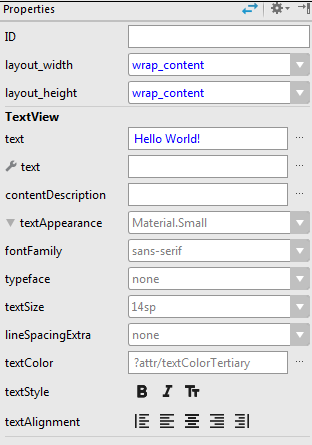
\includegraphics[width=0.8\textwidth]{figures/android20.png}
    \caption{Properties Android Studio}
    \label{print}
    \end{figure}
    
    \item Status Bar
    \par Menampilkan proses pada Android Studio. Proses \textit{Loading, Error,} dan lainnya.
    \begin{figure}[H]
    \centering
    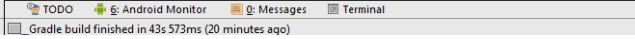
\includegraphics[width=1\textwidth]{figures/android21.png}
    \caption{Status Bar Android Studio}
    \label{print}
    \end{figure}
\end{enumerate}
\subsection{Struktur Folder Project Android Studio}
\par Berikut adalah struktur folder project pada Android Studio :
    \begin{figure}[H]
    \centering
    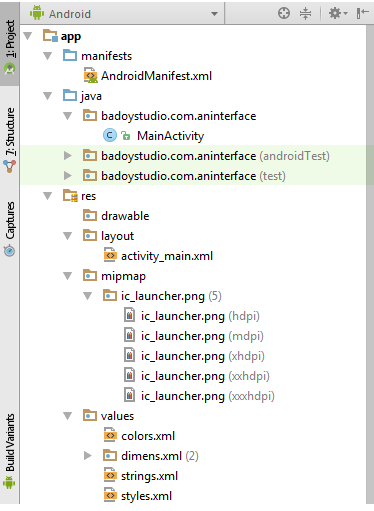
\includegraphics[width=0.8\textwidth]{figures/android22.png}
    \caption{Struktur Folder Projectr Android Studio}
    \label{print}
    \end{figure}
    
    \begin{enumerate}
        \item Manifests 
        \par AndroidManifest.xml :  File ini digunakan untuk melakukan beberapa pengaturan seperti nama aplikasi, icon aplikasi, \textit{theme style } dan \textit{User permission} (jika membuat aplikasi yang membutuhkan akses hardware smartphone ataupun koneksi internet ).
        \item Java
        \par MainActivity.java : digunakan untuk memberikan perintah agar aplikasi melakukan sesuatu menggunakan bahasa pemrograman java.
        \item Res Drawable
        \par Folder yang digunakan untuk memasukan gambar pendukung aplikasi yang kita buat baik berupa icon ataupun lainnya
        \item Res Layout
        \par activitymain.xml : digunakan utuk pengaturan layout untuk interface utama pada aplikasi android yang kita buat.
        \item mipmap
        \par Folder ini digunakan untuk memasukan gambar berupa icon. Icon default aplikasi yang kita buat juga diambil dari folder ini.
        \item values 
        \par colors.xml : file ini berisi kode-kode untuk pengaturan warna. Warna status bar, teks, ataupun lainnya. 
        \par dimens.xml : digunakan untuk pengaturan margin aplikasi.
        \par strings.xml : digunakan untuk pengaturan teks-teks aplikasi yang kita buat.
        \par styles.xml : digunakan untuk memberikan nama warna setelah kode-kode warna dimasukan atau disetting pada color.xml.
        \par 
    \end{enumerate}

   

\subsection{ Bahasa Pemograman Java}
\par Java adalah sebuah bahasa pemrograman yang sangat popular yang dikembangkan oleh Sun Microsystems (saat ini dimiliki oleh Oracle). Dikembangkan lama setelah C dan C++, Java menggabungkan banyak fitur-fitur canggih dari bahasa-bahasa canggih tersebut, sambil mengatasi beberapa kelemahan mereka. Walaupun demikian, tingkat kecanggihan bahasa pemrograman bergantung pada \textit{library} mereka. \textit{Library} ini ada untuk membantu para developer untuk membuat aplikasi. Beberapa fitur inti java :
\begin{enumerate}
    \item Mudah dipelajari dan dimengerti.
    \item Didesain untuk tidak bergantung kepada platform dan aman,     menggunakan mesin virtual
    \item Bersifat\textit{ object-oriented} (fokus kepada objek program ketimbang logic)
\end{enumerate}
\par Android sangat bergantung kepada sifat-sifat dasar dari Java tersebut. Android SDK mengandung banyak \textit{library} Java standar (\textit{library} struktur data, \textit{library} matematika, \textit{library} grafik, \textit{library networking }dan apapun yang dapat Anda inginkan) dan juga\textit{ library special }Android yang dapat membantu mengembangkan aplikasi Android yang keren.



\section{Membuat Aplikasi Monitoring \textit{Prototype}}
\par Pada\textit{ prototype} prediksi ketinggian air (PKA) untuk mendeteksi banjir peringatan dini ini dibuat sebuah aplikasi berbasis android.selain notifikasi melalui telegram adanya juga sebuah aplikasi yang digunakan untuk memonitoring ketinggian air agar masyarakat mendapatkan informasi atau data mengenai ketinggian air secara \textit{real time}. \\
\par Untuk membuat sebuah aplikasi monitoring ini menggunakan sebuah software yaitu android studio dengan menggunakan bahasa java, dimana bahasa java sudah dibahas pada bab ini di penjelasan sebelumnya.

\subsection{Membuat \textit{Spalash Screen}}
\par \textit{Splash screen} adalah tampilan pertama program yang muncul sementara sebelum masuk ke menu utama. Berikut langkah-langkahnya:
\begin{enumerate}
    \item Buka aplikasi android studio kemudian pilih \textit{start a new android studio project }.
    \begin{figure}[H]
    \centering
    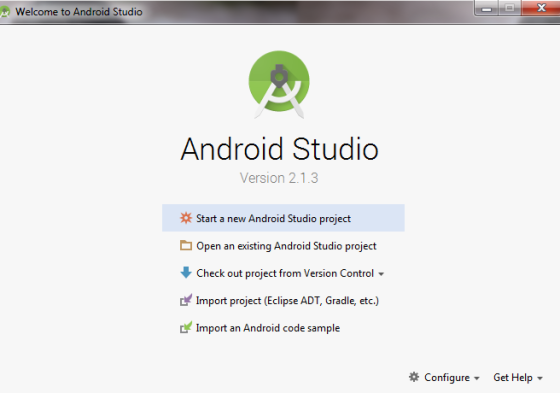
\includegraphics[width=0.7\textwidth]{figures/android23.png}
    \caption{Tampilan Awal Android Studio}
    \label{print}
    \end{figure}
    
    
    \item Pilih \textit{Activity}
    \par \textit{Activity }(aktivitas) adalah sebuah komponen aplikasi yang menyediakan layar yang digunakan pengguna untuk berinteraksi guna melakukan sesuatu, misalnya memilih nomor ponsel, mengambil foto, mengirim email, atau menampilkan peta.

    \par Tiap \textit{ Activity} (aktivitas) diberi sebuah jendela untuk menggambar antarmuka penggunanya. Jendela ini biasanya mengisi layar, namun mungkin lebih kecil daripada layar dan mengambang di atas jendela lain.

    \par Pilih \textit{Empty Activity} kemudian klik Next.
    \begin{figure}[H]
    \centering
    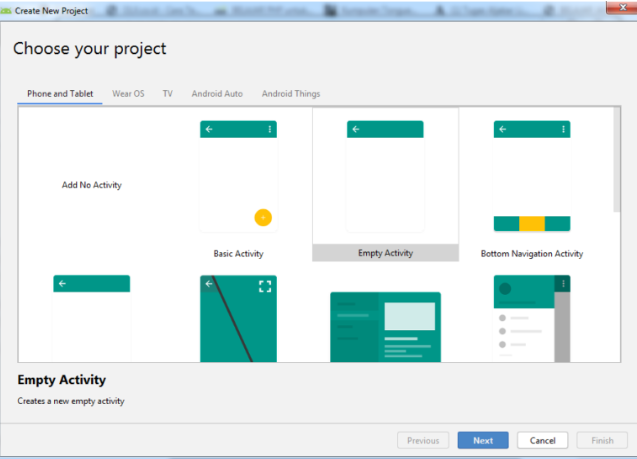
\includegraphics[width=0.7\textwidth]{figures/android24.png}
    \caption{Tampilan Memilih Activity}
    \label{print}
    \end{figure}
    
       \begin{figure}[H]
        \centering
        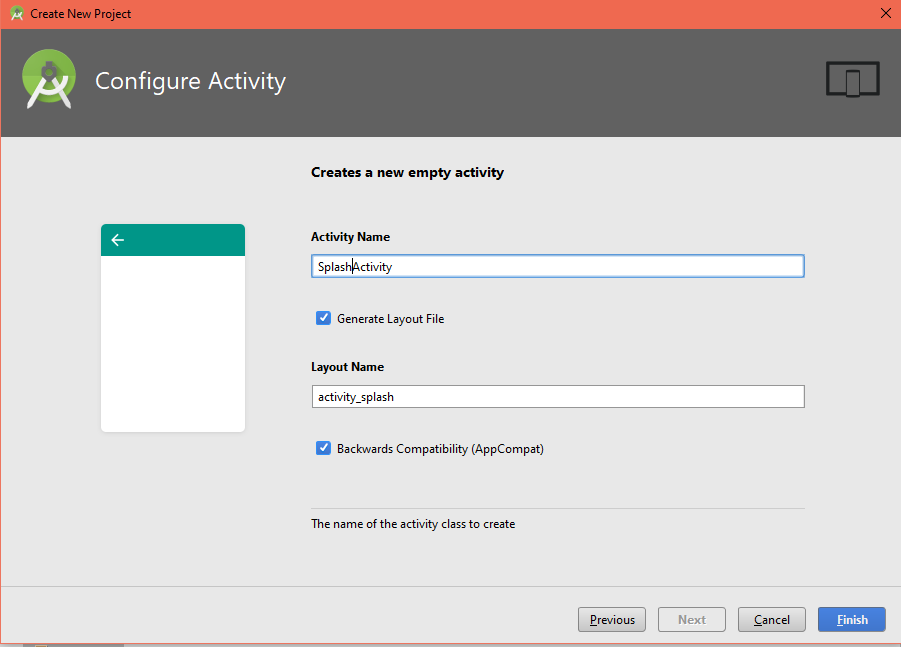
\includegraphics[width=0.7\textwidth]{figures/android27.png}
        \caption{Membuat Activity Spalsh Activity}
        \label{print}
        \end{figure}
    
    \item Konfigurasi \textit{Project}
    Setelah memilih \textit{activity,} langkah selanjutnya yaitu kita harus memberikan konfigurasi pada \textit{project} android yang kita buat. Adapun yang harus di konfigurasi yaitu :
    \begin{enumerate}
        \item Name : isikan nama project
        \item Package name : isikan nama perusahaan atau pembuat aplikasi.
        \item Save location : tentukan file project aplikasi android ini akan disimpan pada direktori apa.
        \item Language : pilih bahasa pemrograman yang akan digunakan, Java atau Kotlin. Pada tutorial ini kita menggunakan Java.
        \item Minimum API level : tentukan API berapa yang akan digunakan. Pada bulan April 2017 google merilis daftar versi OS yang banyak digunakan tahun 2017 dan hasilnya Lollipop (OS versi 5.0 dengan SDK 21/22) ada di urutan nomor satu. Jadi untuk minimum SDKnya kita pilih API 15 yaitu untuk versi OS Ice Cream Sandwich ke atas.
        \begin{figure}[H]
        \centering
        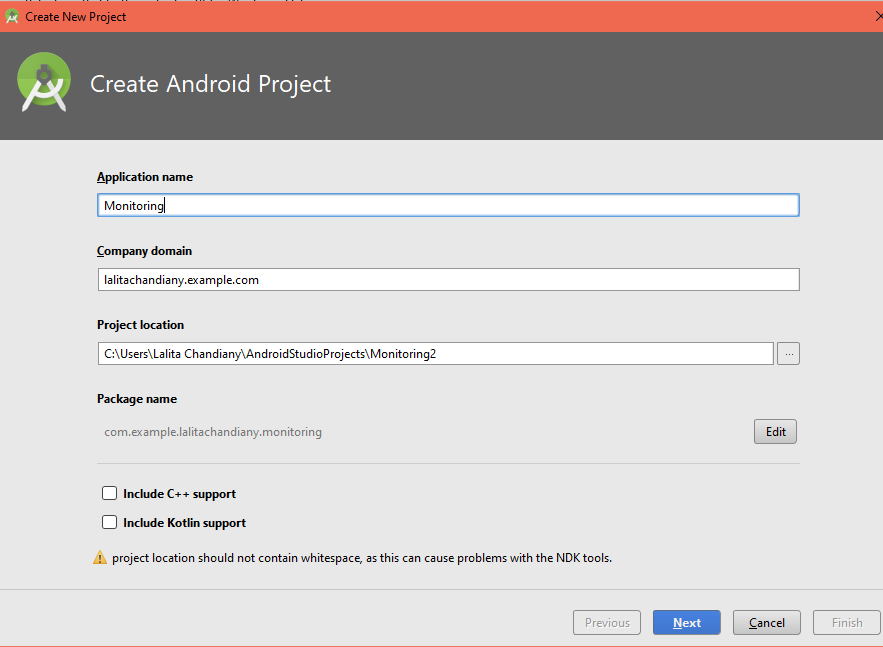
\includegraphics[width=0.9\textwidth]{figures/android25.png}
        \caption{Konfigurasi Project}
        \label{print}
        \end{figure}
        
         \begin{figure}[H]
        \centering
        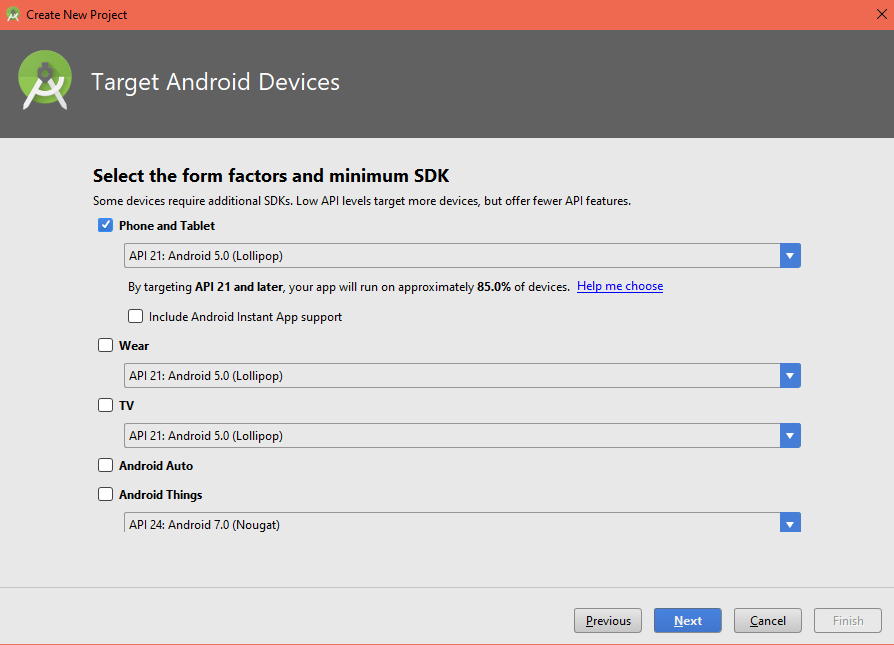
\includegraphics[width=0.9\textwidth]{figures/android26.png}
        \caption{Konfigurasi Project}
        \label{print}
        \end{figure}
  
    \end{enumerate}
      \item  Proses Gradle 
    \begin{figure}[H]
        \centering
        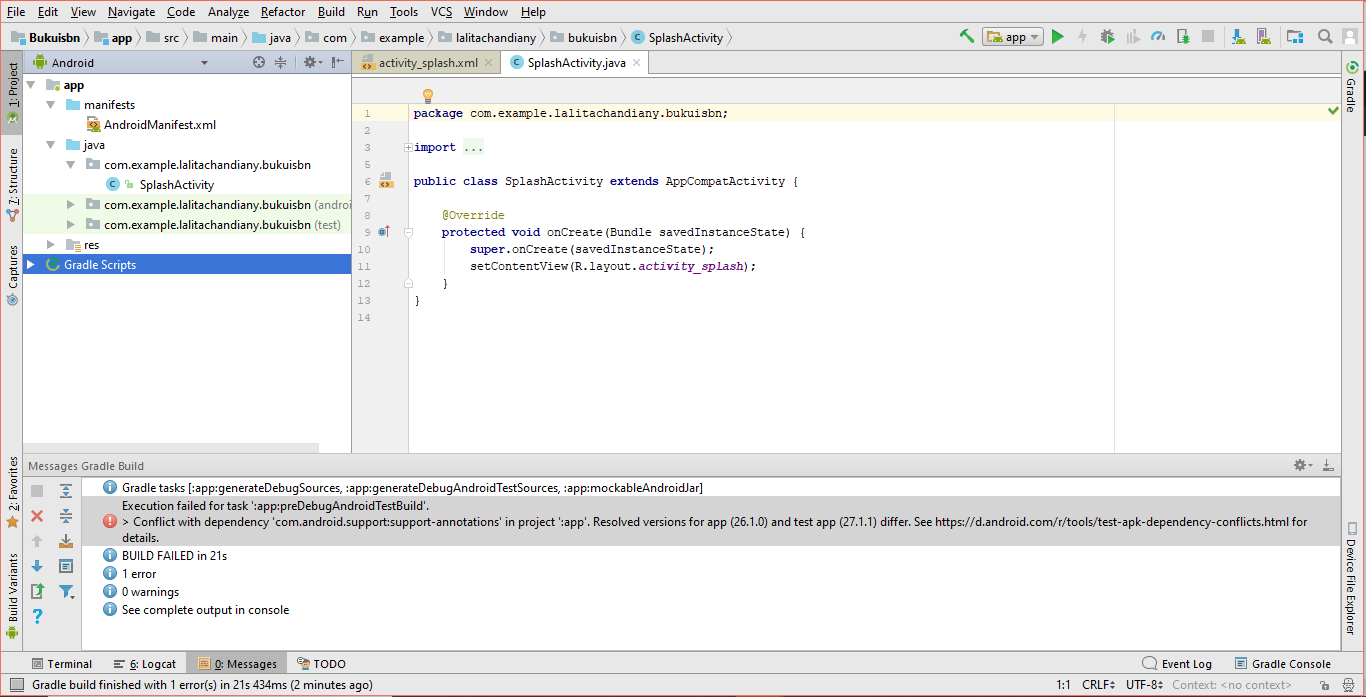
\includegraphics[width=0.9\textwidth]{figures/android28.png}
        \caption{Proses Gradle}
        \label{print}
        \end{figure}
    \pqr Jika pertama kali tampilan di android studio error maka yang bermasalah yaitu mengenai gradlenya untuk mengatasinya yaitu harus menyesuaikan verisnya. Dengan cara mengubah versi gradlenya sesuai dengan apa yang diminta oleh android studio. Untuk menggantinya masuk ke GradleScript-build gradle dan ubah versinya dibagian yang telah dilingkari seperti gambar berikut ini :
    \begin{figure}[H]
        \centering
        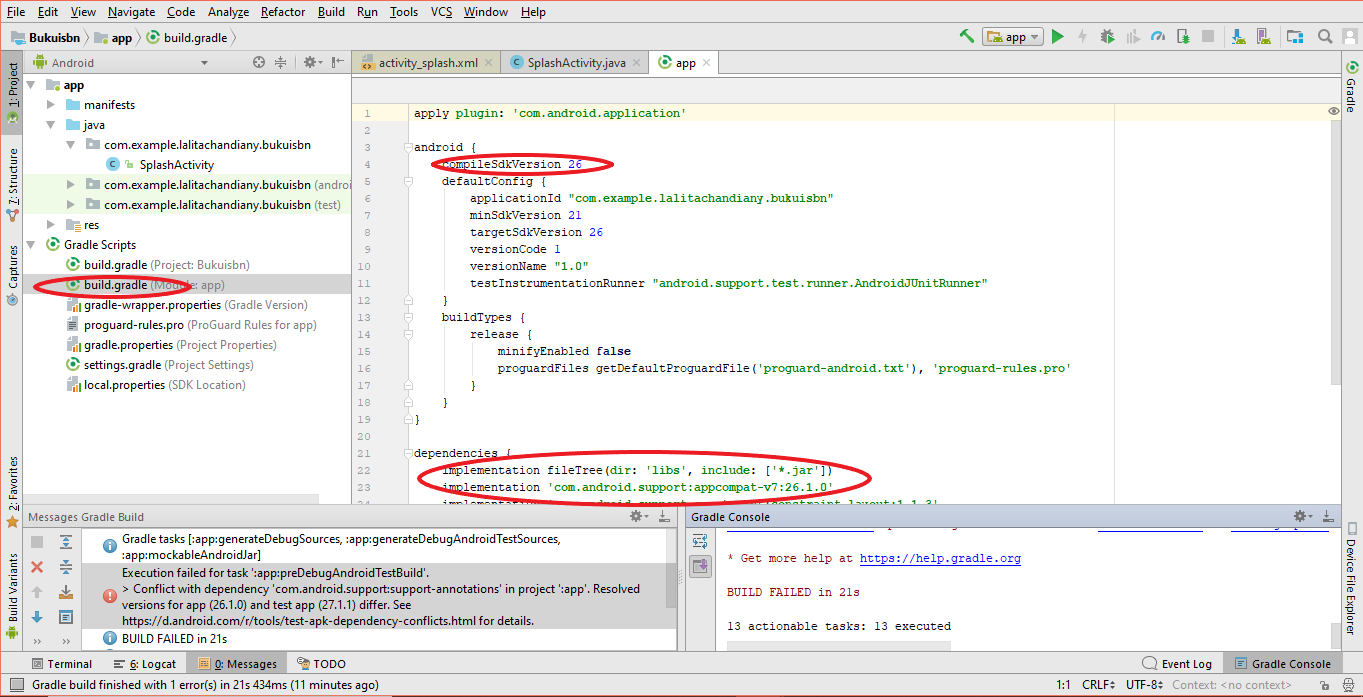
\includegraphics[width=0.9\textwidth]{figures/android29.png}
        \caption{Build Gradle}
        \label{print}
        \end{figure}
    
    \par Tunggu sampai proses gradle selesai. Ini biasanya memakan waktu beberapa menit. Lama atau sebentarnya tergantung spesifikasi ram dan prosesor yang digunakan pada komputer atau laptop.
    
    \item Workspace Android Studio
    \par Jika proses Gradle telah selesai, maka akan terbuka workspace project Android Studio seperti gambar dibawah ini ( pertama kali terbuka adalah tab SplashActivity.java. Disinilah nantinya kita memberikan kode-kode java agar aplikasi bisa melakukan sebuah perintah).
        \begin{figure}[H]
        \centering
        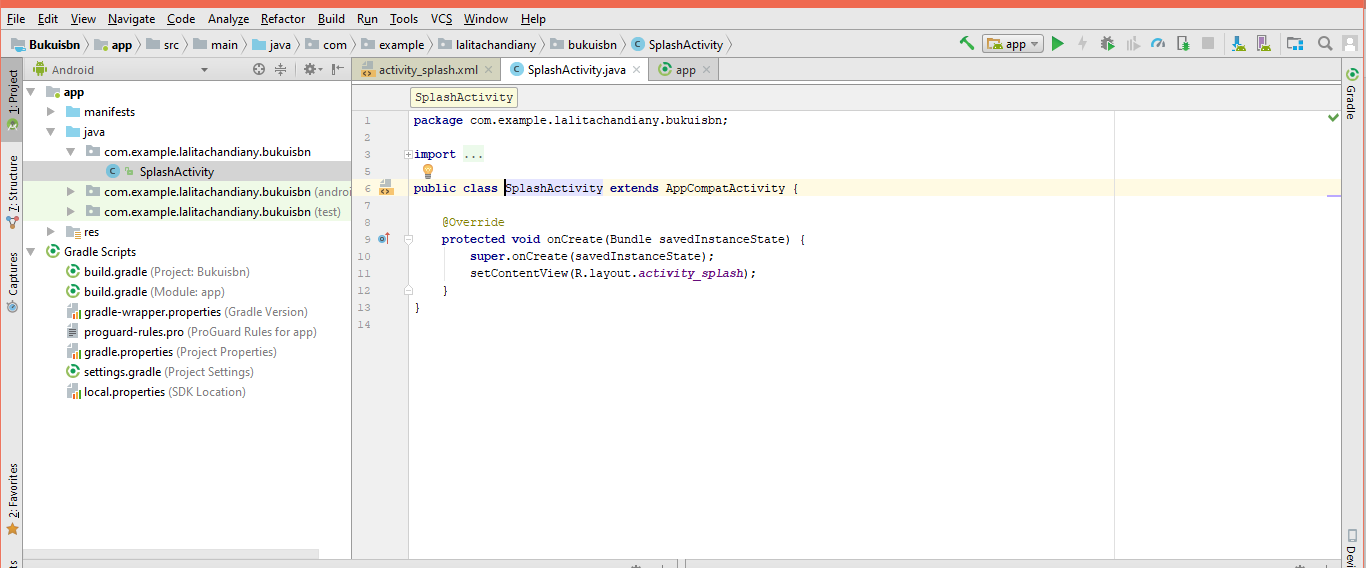
\includegraphics[width=0.9\textwidth]{figures/android30.png}
        \caption{Workspace}
        \label{print}
        \end{figure}
    
    \par Masukan kode berikut ini untuk membuat splash screen di SpalshActivity.java
\lstinputlisting{src/splash.java}

\par Kemudian untuk tampilan Splashscreenya kita harus memasukan gambar yang akan digunakan kedaam folder drawable.
  \begin{figure}[H]
        \centering
        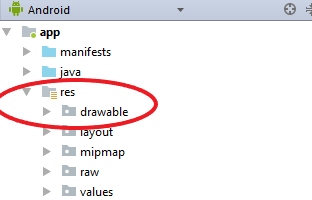
\includegraphics[width=0.9\textwidth]{figures/android31.png}
        \caption{Drawable}
        \label{print}
        \end{figure}
\par Kemudian untuk membuat tampilanya diprogram dalam activityplash.xml dengan kode berikut ini :
\lstinputlisting{src/tampilansplash.xml}
\end{enumerate}

\subsection{ Membuat Halaman Menu}
\par Menu adalah daftar perintah-perintah suatu perangkat lunak (program) yang apabila dieksekusi akan menjalankan suatu perintah tertentu dari aplikasi. Menu digunakan sebagai alternatif dari antarmuka baris perintah. Pilihan yang diberikan oleh menu dapat dipilih dengan menggunakan kursor atau antarmuka pengguna.

\par Dalam menu aplikasi monitoring ini akan adanya slider dan 4 menu utama yaitu \textit{about}, ketinggian air, keterangan air dan \textit{don't panic}. Untuk membuatnya berikut langkah-langkahnya :

\begin{enumerate}
    \item Memnbuat Slider 
    
    \par Slider adalah informasi yang berjalan (sliding) di sebuah aplikasi. Untuk membuatnya hal pertama kali yang harus dilakukan yaitu memasukan gambar apa saja yang akan ditampilkan dengan cara memasukanya kedalam folder drawable.
    
    \par Jika telah memasukan gambar kedalam gradle maka kita import library untuk slider dengan cara memasukan perintahnya di gradle.
    \begin{figure}[H]
        \centering
        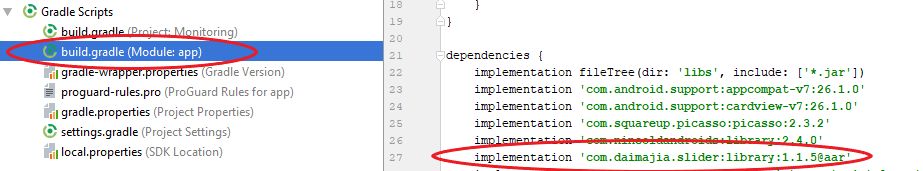
\includegraphics[width=0.9\textwidth]{figures/android32.png}
        \caption{Library Slider}
        \label{print}
        \end{figure}
    \par Setelah memasukan atau \textit{import library} maka kita harus membuat sebuah \textit{activity} baru untuk home. \textit{Activity home} ini akan digunakan untuk 4 menu dan slider yang telah dijelaskan sebelumnya untuk membuat \textit{activity} klik file-new-activity-empaty activity.
    \begin{figure}[H]
        \centering
        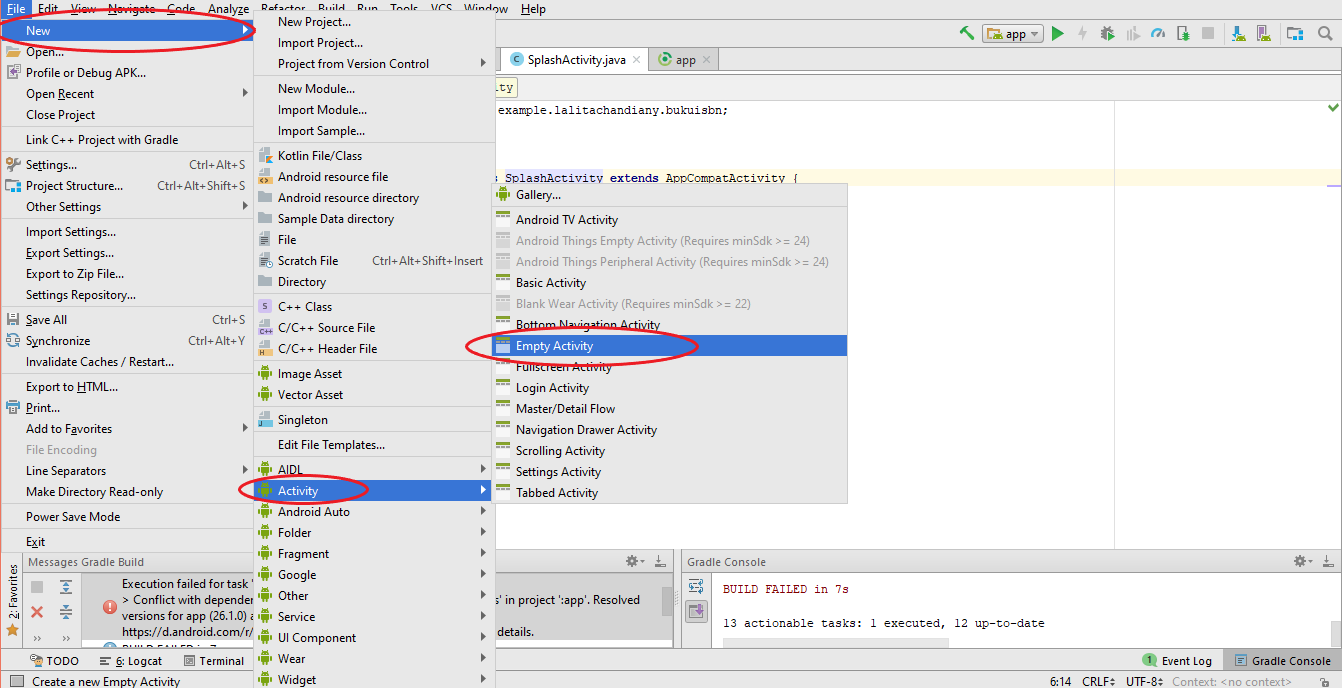
\includegraphics[width=0.9\textwidth]{figures/android33.png}
        \caption{Activity Baru}
        \label{print}
        \end{figure}
        
    \par Jika kita telah membuat \textit{activity} baru maka masukan kode berikut ini kedalam file home.java
\lstinputlisting{src/slider.java}

\par Kemudian untuk tampilanya masukan kode berikut ini kedalam file homeactivity.xml.
\lstinputlisting{src/tampilanslider.xml}

\par Maka hasil nya seperti berikut ini :
\begin{figure}[H]
        \centering
        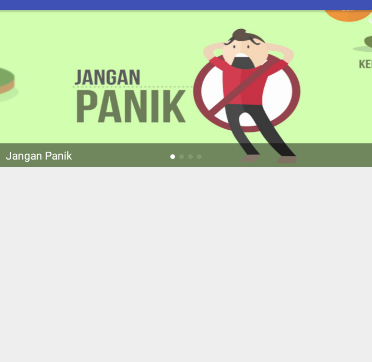
\includegraphics[width=0.7\textwidth]{figures/android34.png}
        \caption{Tampilan Slider}
        \label{print}
        \end{figure}
\item Membuat Menu Di \textit{Home}
\par Dalam aplikasi monitoring ini terdapat 4 menu yaitu menu \textit{about}, ketinggian air, keterangan air dan \textit{don't panic}. Untuk membuat menu ini kita tidak perlu membuat \textit{activity} baru karna menu ini akan ditampilkan secara bersamaan dengan slider, maka kita memprogramnya di \textit{activity home}. 

\par Hal yang harus pertama dilakukan yaitu mengimport \textit{library cardview} karna untuk membuat menu ini dibutuhkan sebuah \textit{library cardview}. Caranya sama dengan langkah sebelumnya dan masukan perintah seperti dibawah ini :
        \begin{figure}[H]
        \centering
        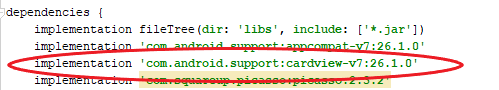
\includegraphics[width=0.7\textwidth]{figures/android35.png}
        \caption{Library Cardview}
        \label{print}
        \end{figure}
\par Jika telah memasukan \textit{library cardview} maka masukan gambar yang akan dijadikan sebagai icon menu ke drawable dengan cara yang sama seperti sebelumnya. Setelah itu masukan kode berikut kedalam file Home.java.
\lstinputlisting{src/menu.java}
\par Jika digabungakan dengan \textit{code} slider sebelumnya maka seperti berikut:
\lstinputlisting{src/homefull.java}

\par Setelah itu untuk tampilanya tambahkan \textit{code} berikut ini kedalam file activityhome.xml.
\lstinputlisting{src/tampilanmenu.xml}
\par Jika digabungakan dengan \textit{code} slider sebelumnya maka seperti berikut:
\lstinputlisting{src/menufull.xml}
\end{enumerate}

\subsection{Membuat Menu \textit{About}}
\par Menu About yaitu menu yang berisi tentang sebab akibat terjadinya banjir. Dimana informasi tersebut disajikan melalui video dan tulisan.
\par langkah pertama yaitu harus membuat sebuah \textit{activity} baru yang diberi nama \textit{about}. Kemudian masukan video yang akan digunakan kedalam folder raw.

\par Kemudian masukan \textit{code} berikut ini kedalam file about.java
\lstinputlisting{src/about.java}
\par Untuk tampilanya masukan \textit{code} berikut ini kedalam file activityabout.xml
\lstinputlisting{src/aboutfull.xml}

\subsection{Membuat Menu Ketinggian Air}
\par Menu ketingian air merupakan sebuah menu untuk menampilkan informasi mengenai ketinggian air yang dibaca oleh sensor jarak secara realtime. 

\par Langkah pertama kita harus mendwonload library antares dengan cara berikut :
\begin{enumerate}
    \item Login ke antares kemudian pilih \textit{documentation} lalu pilih android dan \textit{go to tutorial}
    \item Kemudian \textit{dwonload library} denga cara memilih \textit{dwonload}.
    \begin{figure}[H]
        \centering
        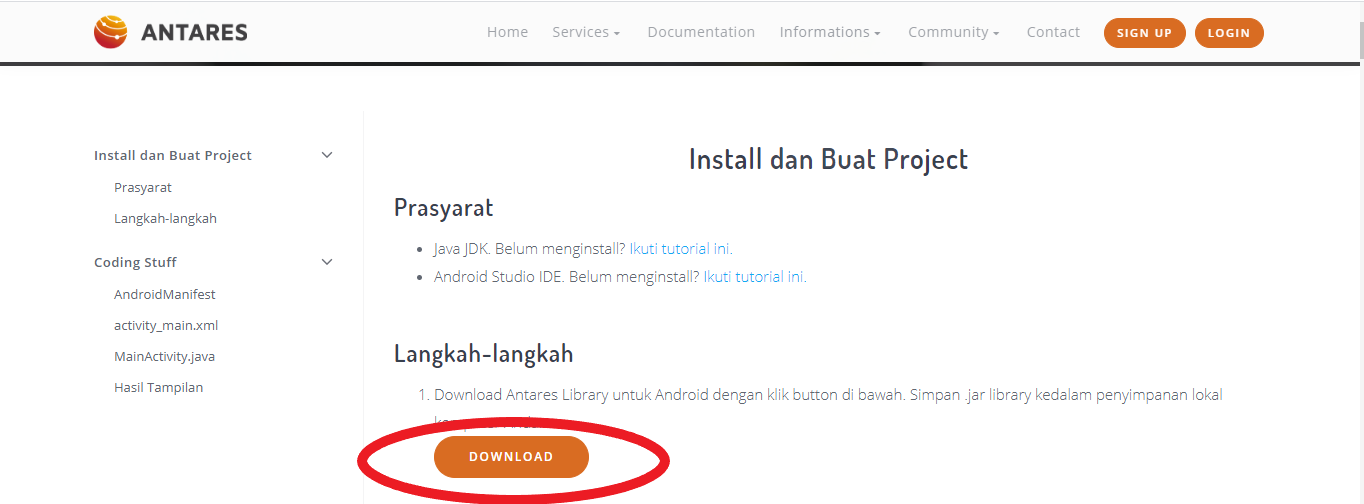
\includegraphics[width=0.9\textwidth]{figures/android36.png}
        \caption{Library Antares}
        \label{print}
        \end{figure}
    \item Setelah itu masukan \textit{library} yang telah di\textit{dwonload} ke folder libs yang ada di android studio.Klik pada bagian android kemudian pilih libs.
    \begin{figure}[H]
        \centering
        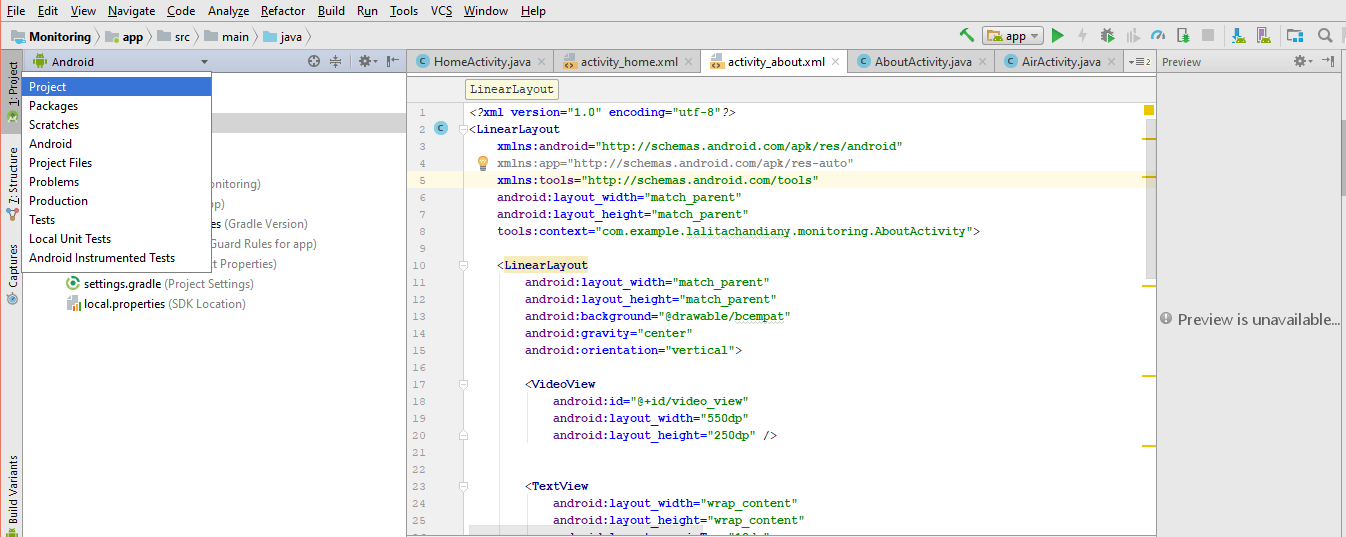
\includegraphics[width=0.9\textwidth]{figures/android37.png}
        \caption{Cara Masuk ke Folder Libs}
        \label{print}
        \end{figure}
    \item Setelah itu \textit{copy-Paste library} jar yang telah didownload ke app -libs. Maka jika sudah \textit{copy - paste} tampilanya seperti berikut.
    \begin{figure}[H]
        \centering
        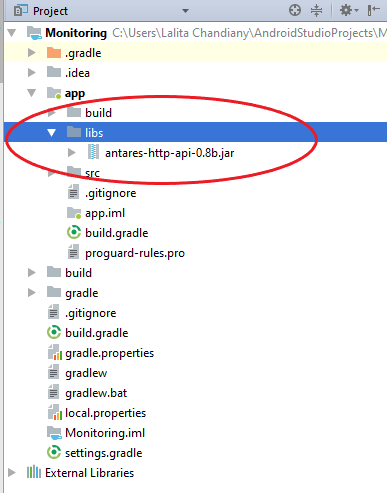
\includegraphics[width=0.9\textwidth]{figures/android39.png}
        \caption{Tampilan Folder Libs}
        \label{print}
        \end{figure}
    \item Agar bisa mengeksekusi API Antares, dibutuhkan akses Internet dan agar bisa mengakses Internet di Android, kita harus tambahkan baris berikut di AndroidManifest.xml.
   \lstinputlisting{src/manifest.java} 
   
   \item Kemudian buat \textit{activity} baru dengan nama monitring. \textit{Activity} ini bertujuan untuk menu ketinggian air. Lalu masukan \textit{code} berikut kedalam file monitoring.java
   \lstinputlisting{src/monitoring.java}
   \item Kemudian untuk tampilan nya masukan \textit{code} berikut kedalam file activitymonitoring.xml
  \lstinputlisting{src/tampilanmon.xml}
\end{enumerate}
\subsection{Membuat Menu Keterangan Air}
\par Menu keterangan air merupakan sebuah menu yang apabila di klik akan menampilkan sebuah halaman yang berisi tentang keterangan level-level ketingian air.

\par Untuk membuat menu keterangan air ini hal yang pertama kali harus dibuat yaitu membuat sebuah \textit{activity} baru dengan nama ketinggian air. Kemudian masukan \textit{code} berikut kedalam file  ketinggianair.java
\lstinputlisting{src/air.java}
\par Kemudian untuk tampilan menu ketinggian airnya masukan perintah berikut di file activityketinggianair.xml
\lstinputlisting{src/tampilanair.xml}

\subsection{Membuat Menu \textit{Don't Panic}}
\par Pada menu \textit{don't ponic} ini akan menampilkan sebuah video dan text yang berisi tentang langkah-langkah apa saja yang harus dilakukan ketika datangnya banjir. Isi pada menu ini bertujuan agar \textit{user} tidak panik dan tau apa yang harus dilakukan ketika banjir datang.

\par Untuk membuatnya sama seperti langkah sebelumnya yaitu membuat \textit{activity} baru dengan nama \textit{panic} , kemudian masukan \textit{code} ke file panic.java sebagai berikut :
\lstinputlisting{src/panic.java}
\par Kemudian untuk tampilan menu \textit{don't pannic} masukan perintah berikut di file panic.xml
\lstinputlisting{src/tampilanpanic.xml}

\section{Tampilan Aplikasi Monitoring}
\par Tampilan dari aplikasi monitoring yang sebelumnya telah dibuat, jika mengikuti semua langkah-langkahnya tanpa adanya step yang terlewatkan maka akan menjadi seperti berikut :

\begin{figure}[H]
        \centering
        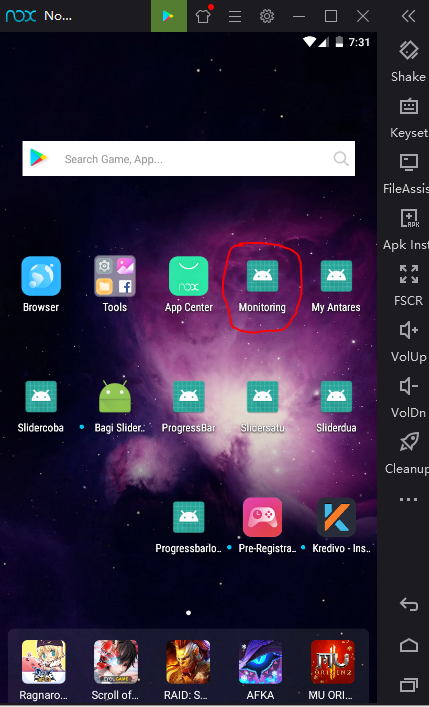
\includegraphics[width=0.5\textwidth]{figures/nox.png}
        \caption{Tampilan Aplikasi DI Emulator}
        \label{print}
        \end{figure}

\begin{figure}[H]
        \centering
        
\includegraphics[width=0.3\textwidth]{figures/satu.png}
        \caption{Splash Screen}
        \label{print}
        \end{figure}
\begin{figure}[H]
        \centering
        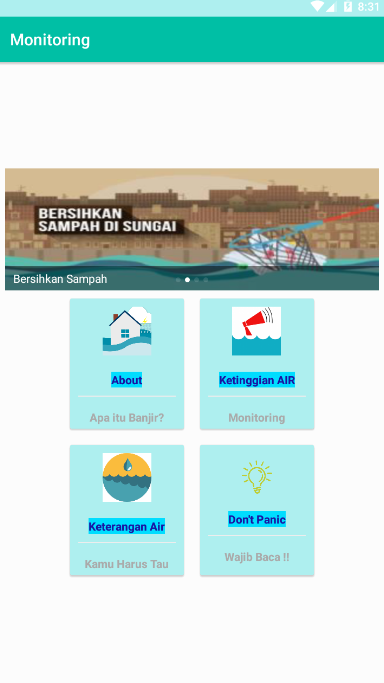
\includegraphics[width=0.4\textwidth]{figures/dua.png}
        \caption{Tampilan Menu Utama}
        \label{print}
        \end{figure}
\begin{figure}[H]
        \centering
        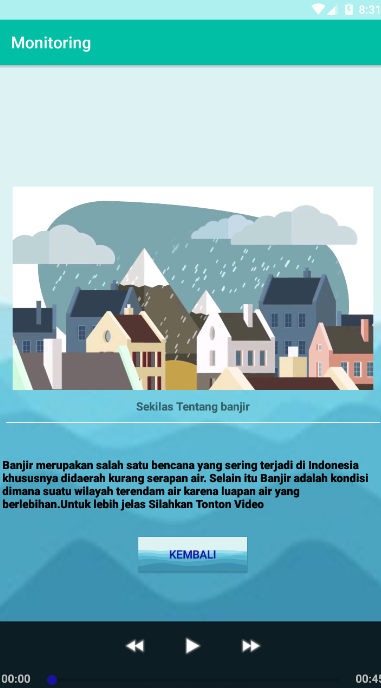
\includegraphics[width=0.3\textwidth]{figures/tiga.png}
        \caption{Tampilan Menu About}
        \label{print}
        \end{figure}
\begin{figure}[H]
        \centering
        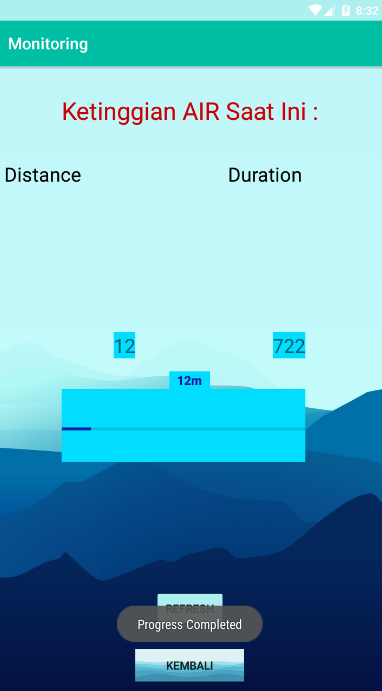
\includegraphics[width=0.4\textwidth]{figures/empat.png}
        \caption{Tampilan Ketinggian Air}
        \label{print}
        \end{figure}
\begin{figure}[H]
        \centering
        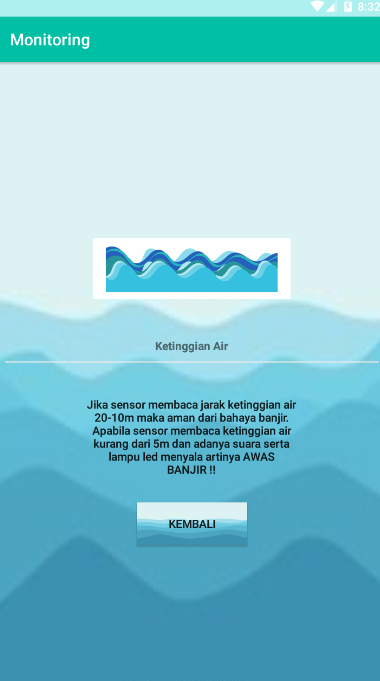
\includegraphics[width=0.3\textwidth]{figures/lima.png}
        \caption{Tampilan Menu Keterangan Air}
        \label{print}
        \end{figure}
\begin{figure}[H]
        \centering
        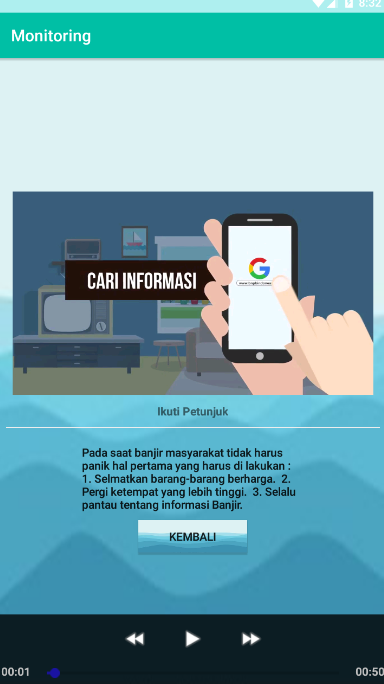
\includegraphics[width=0.4\textwidth]{figures/enam.png}
        \caption{Tampilan Menu \textit{Don't Panic}}
        \label{print}
        \end{figure}
\begin{figure}[H]
        \centering
        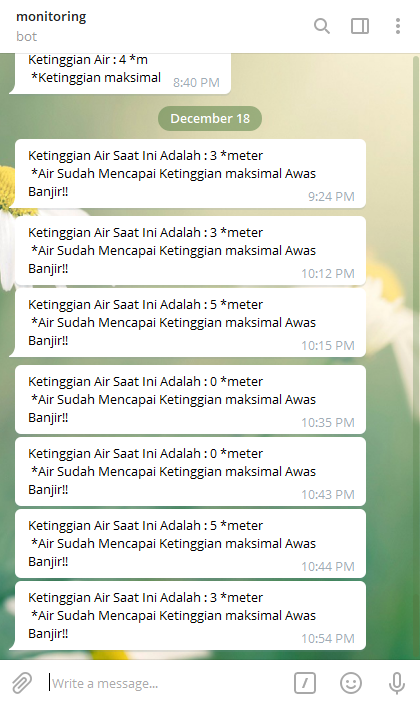
\includegraphics[width=0.5\textwidth]{figures/telegram2.png}
        \caption{Tampilan Notifikasi Telegram}
        \label{print}
        \end{figure}